%------------------------------------------------------------------------
% Presentation example for students by Markus Koschi
%
% compile with LaTeX + dvips + ps2pdf or 
% compile with PdfLaTeX after removing all eps figures 

%------------------------------------------------------------------------
\documentclass[shortpres,aspectratio=43]{beamer}
%\documentclass[shortpres,aspectratio=169]{beamer}
\usetheme{CambridgeUS}


\setbeamertemplate{footline}
{
  \leavevmode%
  \hbox{%
  \begin{beamercolorbox}[wd=.333333\paperwidth,ht=2.25ex,dp=1ex,left]{author in head/foot}%
  \hspace*{4ex}\usebeamerfont{author in head/foot}\insertshortauthor%~~\beamer@ifempty{\insertshortinstitute}{}{(\insertshortinstitute)}
  \end{beamercolorbox}%
  \begin{beamercolorbox}[wd=.333333\paperwidth,ht=2.25ex,dp=1ex,center]{title in head/foot}%
    \usebeamerfont{title in head/foot}\insertshorttitle
  \end{beamercolorbox}%
  \begin{beamercolorbox}[wd=.333333\paperwidth,ht=2.25ex,dp=1ex,right]{date in head/foot}%
    %\usebeamerfont{date in head/foot}\insertshortdate{}\hspace*{2em}
    \insertframenumber{} / \inserttotalframenumber\hspace*{2ex}
  \end{beamercolorbox}}%
  \vskip0pt%
}\part{title}
\beamertemplatenavigationsymbolsempty

%color specification-----------------------------------------------------
\definecolor{TUMblue}{RGB}{27, 94, 170}%{rgb}{0.00, 0.40, 0.74}
\definecolor{TUMgray}{rgb}{0.85, 0.85, 0.86}
\definecolor{TUMpantone285C}{rgb}{0.00, 0.45, 0.81}
\definecolor{TUMpantone300C}{RGB}{27, 94, 170} %uncorrected TUMpantone300C
\definecolor{lightblue}{RGB}{213,227,241}%{rgb}{0.7529,0.8118,0.9333}

\setbeamercolor{block title}{fg=white, bg=TUMblue}
\setbeamercolor{block body}{bg=lightblue}
\setbeamertemplate{blocks}[rounded][shadow=true]

%------------------------------------------------------------------------
\setbeamercolor{frametitle}{bg=TUMblue, fg=white}
\setbeamercolor{palette primary}{bg=TUMblue, fg=white}%{fg=TUMblue,bg=TUMgray}
\setbeamercolor{palette secondary}{use=palette primary,bg=TUMblue, fg=white}
\setbeamercolor{palette tertiary}{use=palette primary,fg=white, bg=TUMblue}
\setbeamercolor{palette quaternary}{use=palette primary,fg=white, bg=TUMblue}

\setbeamercolor{title}{bg=TUMblue,fg=white}
\setbeamercolor{item projected}{use=item,fg=black,bg = lightblue}
\setbeamercolor{block title}{fg=black, bg=lightblue}
\setbeamercolor{block body}{bg=white}
\setbeamertemplate{blocks}[rounded][shadow=true]

%------------------------------------------------------------------------
\setbeamertemplate{bibliography item}{\insertbiblabel}
\setbeamercolor{bibliography item}{parent=palette primary}
\setbeamercolor{bibliography entry author}{fg=TUMblue}

%------------------------------------------------------------------------
\usepackage{subfigure}
\usepackage{textpos} % for figure (logo) on slides
\usepackage{psfrag} % for \psfrag in figures
%\usepackage{algorithm,algpseudocode} % for algorithm environment
%\usepackage{booktabs} % for rulers in tables
\usepackage{units} % for units to values
\usepackage{media9}
%\usepackage{hyperref}
%\usepackage{graphicx}

%-----------------------------------------------------------------------
\newcommand{\at}{\fontfamily{ptm}\selectfont @}
\newcommand{\ra}[1]{\renewcommand{\arraystretch}{#1}} %to change the row spacing in tables

\newcommand\blfootnote[1]{%
  \begingroup
  \renewcommand\thefootnote{}\footnote{#1}%
  \addtocounter{footnote}{-1}%
  \endgroup
}

%-----------------------------------------------------------------------
\title[Title]{Realistic Optimization-based Driving Using a Constrained Double-Integrator Model}

\author[Name]{Andreas Belavic}
\institute[TU M\"unchen]{Technical University of Munich}

\date{March~31,~2025}

%---------------------------------------------------------------------
\begin{document}

%% TUM logo
\addtobeamertemplate{frametitle}{}{%
  \begin{textblock*}{\textwidth}(.91\textwidth,-0.925cm) % for aspectratio=43
    
\includegraphics[height=0.65cm]{./figures/TUM_Logo_weiss_e.eps} % for aspectratio=43
    %\begin{textblock*}{\textwidth}(.92\textwidth,-0.93cm) % for aspectratio=169
    %
\includegraphics[height=0.7cm]{./figures/TUM_Logo_weiss_e.eps} % for aspectratio=169
  \end{textblock*}}

\begin{frame}[plain]
  \titlepage
\end{frame}

% Slide 2: Motivation & Problem Statement
\begin{frame}{Motivation \& Problem Statement}
  \begin{itemize}
    \item Autonomous driving demands safe, real-time trajectory planning.
    \item Balancing model accuracy with computational efficiency is critical.
    \item Our approach uses convex optimization with a constrained double-integrator model.
  \end{itemize}
  \centering
  \textbf{[Placeholder: Schematic diagram of motion planning challenges]}

  \includemedia[
    width=0.6\linewidth,
    height=0.45\linewidth,
    activate=pageopen,
    addresource=/Users/andreasbelavic/bachelor-thesis/code/benchmark-results/elchtest_1-RoadAlignedModel-27-01-2025-13:31:15/animation.mp4,
    flashvars={
        source=/Users/andreasbelavic/bachelor-thesis/code/benchmark-results/elchtest_1-RoadAlignedModel-27-01-2025-13:31:15/animation.mp4  % path to the video file
      }
  ]{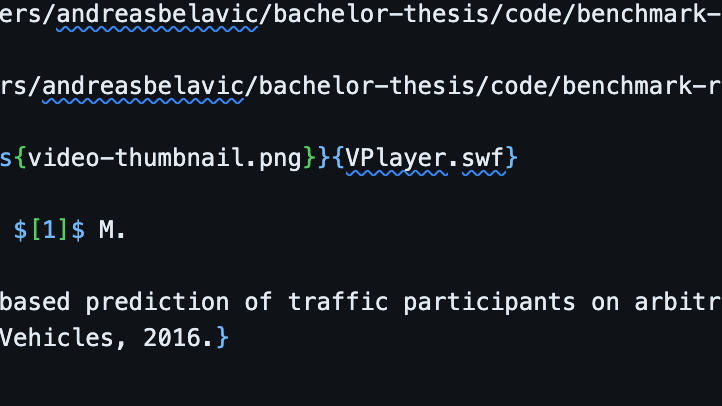
\includegraphics{video-thumbnail.png}}{VPlayer.swf}

  \blfootnote{\tiny $[1]$ M.
    Althoff and S.
    Magdici, ``Set-based prediction of traffic participants on arbitrary road networks,'' IEEE Trans.
    on Intelligent Vehicles, 2016.}
\end{frame}

% Slide 3: Overview of the Approach
\begin{frame}{Overview of the Approach}
  \begin{itemize}
    \item Reformulates trajectory planning as a convex optimization problem.
    \item Simplifies vehicle dynamics via the double-integrator model.
    \item Applies feedback linearization and convex inner approximations.
  \end{itemize}
  \centering
  \textbf{[Placeholder: Block diagram of the planning framework]}
  \blfootnote{\tiny $[2]$ A.
    Belavic, Bachelor’s Thesis, TUM, 2025.
  }
\end{frame}

% Slide 4: Double Integrator Model
\begin{frame}{Vehicle Modeling: Double Integrator Model}
  \begin{itemize}
    \item Simplified dynamics: considers only position and velocity.
    \item Ignores orientation for computational efficiency.
    \item Leads to a convex formulation ideal for real-time planning.
  \end{itemize}
  \centering
  \textbf{[Placeholder: Diagram of double integrator dynamics]}
  \blfootnote{\tiny See Chapter 2 of the thesis.}
\end{frame}

% Slide 5: Kinematic Bicycle Model
\begin{frame}{Vehicle Modeling: Kinematic Bicycle Model}
  \begin{itemize}
    \item Captures vehicle orientation and steering dynamics.
    \item More realistic than the double integrator but computationally heavier.
    \item Often used for validation against simplified models.
  \end{itemize}
  \centering
  \textbf{[Placeholder: Diagram of the bicycle model representation]}
  \blfootnote{\tiny Refer to Chapter 2 for model comparisons.}
\end{frame}

% Slide 6: Coordinate Transformation: Frenet Frame
\begin{frame}{Coordinate Transformation: Frenet Frame}
  \begin{itemize}
    \item Transforms global coordinates into a path-following system.
    \item Simplifies handling of road curvature and lateral deviations.
  \end{itemize}
  \centering
  \textbf{[Placeholder: Illustration of the Frenet frame]}
  \blfootnote{\tiny Adapted from the thesis discussion in Section 2.3.}
\end{frame}

% Slide 7: Framework Architecture
\begin{frame}{Motion Planning Framework Architecture}
  \begin{itemize}
    \item Multi-layered approach: global route, behavioral layer, local trajectory optimization.
    \item Our focus: the local planner using convex optimization.
  \end{itemize}
  \centering
  \textbf{[Placeholder: Block diagram of planning layers]}
  \blfootnote{\tiny Inspired by early work on motion planning architectures [1].}
\end{frame}

% Slide 8: Convex Optimization in Planning
\begin{frame}{Convex Optimization in Motion Planning}
  \begin{itemize}
    \item Ensures smooth and dynamically feasible trajectories.
    \item Allows efficient solution of sub-problems to global optimality.
    \item Supports real-time implementation.
  \end{itemize}
  \blfootnote{\tiny See related discussions in Chapters 3 and 4.}
\end{frame}

% Slide 9: Feedback Linearization
\begin{frame}{Feedback Linearization Technique}
  \begin{itemize}
    \item Linearizes nonlinear vehicle dynamics via state feedback.
    \item Decouples acceleration and steering commands.
    \item Simplifies controller design.
  \end{itemize}
  \centering
  \textbf{[Placeholder: Schematic showing feedback linearization]}
  \blfootnote{\tiny Technique detailed in Section 3.1.4 of the thesis.}
\end{frame}

% Slide 10: Constraint Handling
\begin{frame}{Constraint Handling in the Framework}
  \begin{itemize}
    \item Incorporates physical limits: acceleration, velocity, and road boundaries.
    \item Uses convex inner approximations for non-convex constraints.
    \item Maintains safety and feasibility.
  \end{itemize}
  \centering
  \textbf{[Placeholder: Diagram of constraint mapping]}
  \blfootnote{\tiny Constraint formulations are discussed in Section 3.1.5.}
\end{frame}

% Slide 11: Quantifier Elimination & Convex Approximation
\begin{frame}{Quantifier Elimination \& Convex Approximations}
  \begin{itemize}
    \item Two approaches: interval fitting and Cylindrical Algebraic Decomposition (CAD).
    \item Derives an inscribed polytope for the feasible set.
    \item Balances computational efficiency with accuracy.
  \end{itemize}
  \centering
  \textbf{[Placeholder: Graphical comparison of interval fitting and CAD]}
  \blfootnote{\tiny For details, see Sections 3.1.6 of the thesis.}
\end{frame}

% Slide 12: Simulation Setup
\begin{frame}{Simulation Setup: Implementation Details}
  \begin{itemize}
    \item Road segments, planner configurations, and soft constraints are defined.
    \item Simulation scenarios mimic realistic driving conditions.
    \item Ensures the evaluation is comprehensive.
  \end{itemize}
  \centering
  \textbf{[Placeholder: Table summarizing simulation parameters]}
  \blfootnote{\tiny Implementation details from Section 4.1.}
\end{frame}

% Slide 13: Evaluation Metrics and Scenarios
\begin{frame}{Evaluation Metrics and Scenarios}
  \begin{itemize}
    \item Metrics: trajectory feasibility, computational time, and safety margins.
    \item Multiple scenarios: straight roads, curved segments, and dynamic obstacles.
  \end{itemize}
  \centering
  \textbf{[Placeholder: Diagram or chart of evaluation metrics]}
  \blfootnote{\tiny Refer to Section 4.2 of the thesis.}
\end{frame}

% Slide 14: Numerical Experiment: Scenario 1
\begin{frame}{Numerical Experiment: Scenario 1}
  \begin{itemize}
    \item Scenario: Moderate-speed driving on a straight road.
    \item Result: Smooth trajectory with rapid solver convergence.
  \end{itemize}
  \centering
  \textbf{[Placeholder: Simulation snapshot of Scenario 1]}
  \blfootnote{\tiny Simulation results are detailed in Chapter 4.}
\end{frame}

% Slide 15: Numerical Experiment: Scenario 2
\begin{frame}{Numerical Experiment: Scenario 2}
  \begin{itemize}
    \item Scenario: Handling a sharp curve.
    \item Result: Effective management of lateral deviations.
  \end{itemize}
  \centering
  \textbf{[Placeholder: Simulation snapshot of Scenario 2]}
  \blfootnote{\tiny See performance analysis in Chapter 4.}
\end{frame}

% Slide 16: Computational Efficiency
\begin{frame}{Performance: Computational Efficiency}
  \begin{itemize}
    \item Optimization runs in real time under dynamic conditions.
    \item Solver times validate the framework's efficiency.
  \end{itemize}
  \centering
  \textbf{[Placeholder: Plot of solver runtime vs. scenario complexity]}
  \blfootnote{\tiny Performance evaluation from Section 4.2.}
\end{frame}

% Slide 17: Model Comparison
\begin{frame}{Comparison: Double Integrator vs. Bicycle Model}
  \begin{itemize}
    \item Double integrator: Fast and efficient, less detailed.
    \item Bicycle model: Higher fidelity but increased computational load.
    \item Trade-offs guide model selection based on application needs.
  \end{itemize}
  \centering
  \textbf{[Placeholder: Comparative table/graph]}
  \blfootnote{\tiny Comparison drawn from Chapter 2 and related literature.}
\end{frame}

% Slide 18: Advantages of the Framework
\begin{frame}{Advantages of the Proposed Framework}
  \begin{itemize}
    \item Convex formulation ensures global optimality within sub-problems.
    \item Robust to dynamic environmental changes.
    \item Provides a foundation for scalable autonomous driving solutions.
  \end{itemize}
  \blfootnote{\tiny Advantages summarized in the thesis conclusion.}
\end{frame}

% Slide 19: Limitations and Challenges
\begin{frame}{Limitations and Challenges}
  \begin{itemize}
    \item Trade-off: Simplified models may sacrifice some accuracy.
    \item Conservative approximations can limit optimality.
    \item Extension to highly dynamic scenarios remains challenging.
  \end{itemize}
  \centering
  \textbf{[Placeholder: Diagram illustrating limitations]}
  \blfootnote{\tiny Challenges discussed in Chapter 5.}
\end{frame}

% Slide 20: Future Work
\begin{frame}{Future Work and Extensions}
  \begin{itemize}
    \item Incorporate full dynamic models for enhanced accuracy.
    \item Integrate with sensor data for real-world validation.
    \item Develop adaptive control strategies to improve performance.
  \end{itemize}
  \centering
  \textbf{[Placeholder: Flowchart of future research directions]}
  \blfootnote{\tiny Future work is outlined in the thesis conclusion.}
\end{frame}

% Slide 21: Key Findings
\begin{frame}{Key Findings and Contributions}
  \begin{itemize}
    \item Proposed a convex optimization framework for motion planning.
    \item Demonstrated realistic, safe trajectories with a constrained double-integrator.
    \item Validated through extensive simulations and performance evaluations.
  \end{itemize}
  \blfootnote{\tiny Key contributions summarized in Chapter 5.}
\end{frame}

% Slide 22: Impact on Autonomous Driving
\begin{frame}{Impact on Autonomous Driving}
  \begin{itemize}
    \item Enhances real-time trajectory planning capabilities.
    \item Improves safety and efficiency in autonomous vehicle operations.
    \item Lays groundwork for further advancements in motion planning.
  \end{itemize}
  \blfootnote{\tiny Impact discussed in the thesis discussion section.}
\end{frame}

% Slide 23: Discussion and Q\&A Preparation
\begin{frame}{Discussion and Q\&A Preparation}
  \begin{itemize}
    \item How does convex approximation affect optimality?
    \item What are the trade-offs of using a double-integrator model?
    \item How scalable is the approach for complex, dynamic scenarios?
  \end{itemize}
  \centering
  \textbf{[Placeholder: List of potential discussion questions]}
  \blfootnote{\tiny Questions based on open issues in Chapters 4 and 5.}
\end{frame}

% Slide 24: Summary and Final Thoughts
\begin{frame}{Summary and Final Thoughts}
  \begin{itemize}
    \item Reviewed the modeling, optimization, and simulation of our framework.
    \item Highlighted benefits, limitations, and future research directions.
    \item Emphasized the importance of real-time feasibility and safety.
  \end{itemize}
  \centering
  \textbf{[Placeholder: Summary diagram of the presentation]}
  \blfootnote{\tiny Summary adapted from the thesis conclusion.}
\end{frame}

% Slide 25: Conclusions
\begin{frame}{Conclusions}
  \begin{itemize}
    \item Presented a comprehensive, convex optimization framework for motion planning.
    \item Balanced computational efficiency with realistic vehicle dynamics.
    \item Contributed to advancing motion planning in autonomous driving.
  \end{itemize}
  \centering
  \textbf{[Placeholder: Final summary graphic]}
  \blfootnote{\tiny Conclusions drawn from the overall thesis work.}
\end{frame}

\end{document}